\chapter{Manual de utilización}
\label{Anexo:manualuso}
En este apartado se detallarán todos los aspectos necesarios para la ejecución y el correcto funcionamiento del proyecto. Se guiará al usuario a través de todo el proceso, desde la instalación del software necesario hasta todas las utilidades que tienen que ver con el workflow, pasando por una breve guía de uso de \textit{Galaxy} orientada a nuestro caso.
\section{Requisitos}

\begin{table}[!h]

\begin{center}
\begin{tabularx}{\textwidth}{bs}
\arrayrulecolor{NavyBlue}\hline
\multicolumn{2}{l}{%
\textbf{\textcolor{NavyBlue}{Requisitos hardware}}}\\
\quad 15 GB de espacio libre en disco \\

\quad 16 GB de memoria RAM \\

\quad procesador de 4 núcleos a 2.5 Ghz (recomendado) \\

\arrayrulecolor{NavyBlue}\hline
\multicolumn{2}{l}{%
\textbf{\textcolor{NavyBlue}{Requisitos software}}} \\
\quad Sistema \textit{Ubuntu} (recomendada versión cercana a la 18.04) \\

\quad \textit{Docker} 18.09.1 o superior\\

\hline

\end{tabularx}
\end{center}
\label{table:Requisitos sistema}
\caption{Requisitos del sistema}
\end{table}
En primer lugar, debido a la complejidad de las ejecuciones y al gran tamaño de la imagen \textit{Galaxy} y de los datos de entrada de las ejecuciones, se requiere de unos componentes hardware relativamente exigentes~\ref{table:Requisitos sistema}. Una de las herramientas utilizadas en el workflow, \textit{SPAdes}, necesita cargar gran cantidad de datos en memoria RAM, por lo que se recomienda una capacidad de 16 GB. Se requiere, también, de 20 GB de espacio libre en disco para almacenar cómodamente la imagen \textit{Galaxy} y los datos que se utilicen. El procesador es un aspecto menos restrictivo, pero las ejecuciones serán más lentas con peores procesadores. Como orientación, en un procesador de 8 núcleos a 3.6 Ghz, una ejecución con unos 10 GB de datos de entrada, tarda aproximadamente 3 horas.

En cuanto al software~\ref{table:Requisitos sistema}, el primer requisito es un sistema operativo Linux. Preferiblemente una versión cercana a \textit{Ubuntu 18.04.1}, la utilizada para el desarrollo.

También será necesario disponer de \textit{Docker} en el equipo. Si no está instalado, en el apartado de <<Instalación de \textit{Docker}>> a continuación, se detallará el proceso a realizar.

\section{Utilización}
\subsection{Instalación de Docker}
Partiendo de un sistema \textit{Ubuntu}, lo primero que deberemos instalar será \textit{Docker}. Para ello, abriremos la terminal de \textit{linux} y seguiremos el tutorial de su web oficial\footnote{\url{https://docs.docker.com/install/linux/docker-ce/ubuntu/}}. El primer paso será actualizar la lista de paquetes disponibles para la instalación. Para ello, escribiremos en la terminal:
    \begin{lstlisting}[language=bash]
    $ sudo apt-get update
    \end{lstlisting}
A continuación, instalaremos varios paquetes que serán necesarios más adelante.
    \begin{lstlisting}[language=bash]
    $ sudo apt-get install \
    apt-transport-https \
    ca-certificates \
    curl \
    gnupg-agent \
    software-properties-common
    \end{lstlisting}
Ahora añadiremos la clave para el repositorio oficial de \textit{Docker} al sistema.
    \begin{lstlisting}[language=bash]
    $ curl -fsSL https://download.docker.com/linux/ubuntu/gpg | \ 
    sudo apt-key add -
    \end{lstlisting}
Necesitaremos añadir el repositorio \textit{Docker}.
    \begin{lstlisting}[language=bash]
    $ sudo add-apt-repository \
   ``deb [arch=amd64] https://download.docker.com/linux/ubuntu \
   $(lsb_release -cs) \
   stable''
    \end{lstlisting}
Antes de finalizar, actualizaremos de nuevo la lista de paquetes disponibles.
    \begin{lstlisting}[language=bash]
    $ sudo apt-get update
    \end{lstlisting}
Finalmente, instalaremos \textit{Docker}.
    \begin{lstlisting}[language=bash]
    $ sudo apt install docker-ce
    \end{lstlisting}
Dado que realizaremos frecuentemente ejecuciones con el comando <<docker>>, añadiremos nuestro usuario al grupo de \textit{Docker} para evitar introducir la clave en cada llamada.
    \begin{lstlisting}[language=bash]
    $ sudo usermod -aG docker ${USER}
    \end{lstlisting}
Para hacerlo efectivo, reiniciaremos nuestra sesión de usuario.
    \begin{lstlisting}[language=bash]
    $ su - ${USER}
    \end{lstlisting}
De esta manera, podremos dar por finalizada la instalación de \textit{Docker}.
\subsection{Descarga de la imagen \textit{Galaxy}}
En la carpeta <<exes>> del proyecto, encontraremos todo lo necesario para interactuar con \textit{Docker} y \textit{Galaxy}. En este caso, para la instalación de la imagen, utilizaremos el script <<run.sh>> que se encargará de buscar la imagen \textit{Galaxy} en nuestro ordenador, descargarla, en caso de que no la encuentre, y desplegarla en un contenedor \textit{Docker}. Para ello, desde la terminal nos situaremos en el directorio <<exes>> y escribiremos:
    \begin{lstlisting}[language=bash]
    $ ./run.sh
    \end{lstlisting}
Tras la ejecución de ese comando, en la terminal debería mostrarse un registro del funcionamiento de \textit{Galaxy}, que podremos cerrar cuando deseemos. Si se quiere comprobar el estado de los contenedores \textit{Docker}, se ejecutará
\begin{lstlisting}[language=bash]
    $ docker ps -a
\end{lstlisting}
Dado que \textit{Galaxy} ya está funcionando, podremos acceder simplemente abriendo cualquier navegador web y escribiendo en la barra de navegación <<\url{http://localhost:8080/}>>.


\subsection{Control del contenedor \textit{Docker}}
En el mismo directorio <<exes>> en el que nos situábamos en el paso anterior encontramos varias utilidades para el control de \textit{Docker}.
\begin{description}
    \item[run.sh] despliega la imagen de \textit{Galaxy} en un contenedor \textit{Docker}. Sobrescribirá la imagen \textit{Galaxy} actual si existe alguna.
    \item[stop.sh] detiene el contenedor \textit{Docker}.
    \item[start.sh] arranca el contenedor si está detenido. Para iniciar \textit{Galaxy}, a excepción de la primera vez, deberá usarse este script.
    \item[remove.sh] elimina el contenedor.
    \item[purge.sh] elimina ficheros temporales de \textit{Docker} que pueden causar problemas de espacio.
\end{description}


\subsection{Funcionamiento del workflow en \textit{Galaxy}}
Aunque existe una utilidad para simplificar el proceso de uso de workflow, explicada en la sección \ref{EjecucionSimplificada}, a continuación analizaremos el uso de de \textit{Galaxy} de la manera estándar.

Desde un navegador web cualquiera, si accedemos a la dirección <<\url{http://localhost:8080/}>>, veremos la página de inicio de \textit{Galaxy}. En ella, tendremos la posibilidad de identificarnos mediante la pestaña <<Login or Register>>. Existe un usuario preestablecido con correo <<admin@galaxy.org>> y contraseña <<admin>>. Una vez identificados como administrador tendremos la posibilidad de acceder a los workflows almacenados desde la pestaña <<Workflow>>. En ella, veremos un listado con todas las opciones posibles, la que nos interesa es <<CJ\_Workflow>>. Si desplegamos utilizando la flecha a la derecha del nombre, podremos acceder a las acciones con las que interaccionaremos con este workflow. La primera de ellas es el modo edición, a través de <<edit>>. 

\begin{figure}[!h]
    \begin{center}
      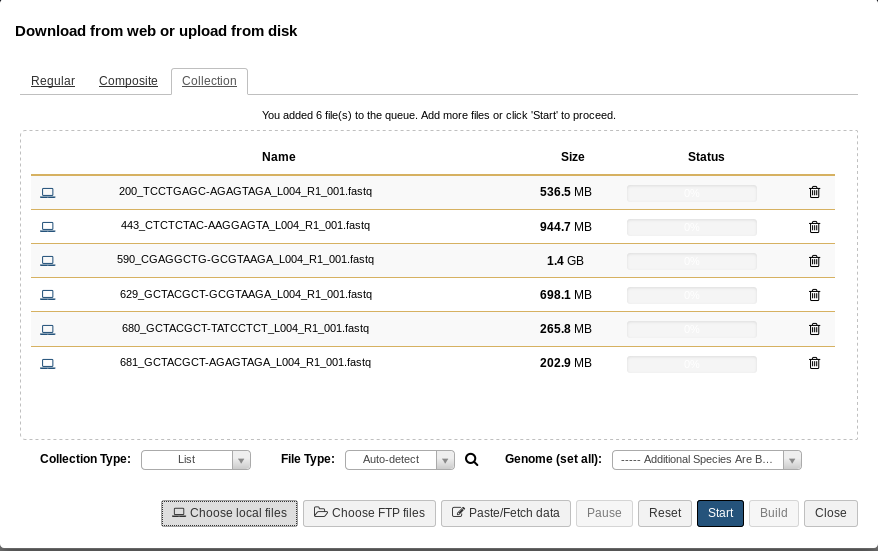
\includegraphics[scale=0.55]{images/SubidaDatasets.png}
      \caption{Interfaz de subida de los conjuntos de datos}
      \label{fig:SubidaDatasets}
    \end{center}
\end{figure}

En la vista de edición~\ref{fig:SubidaDatasets} encontraremos un diagrama formado por las herramientas y uniones que indican las interacciones entre los ficheros de cada una de ellas. Al comienzo del proceso veremos dos cajas con el título <<Input dataset collection>>. Desde este paso se introducirán los datos de entrada al workflow en forma de una estructura denominada colección. Para ver cómo crear esa estructura saldremos un momento de la pestaña workflow, haciendo clic en la opción <<Analyze data>> de la parte superior. A continuación, en el listado de categorías de herramientas que podemos ver en la parte izquierda, abriremos <<Get Data>> seguido de <<Upload File>>. Veremos como se despliega una ventana nueva en la que existen tres opciones de estructuras: <<regular>>, <<composite>> y <<collection>>. Deberemos seleccionar esta tercera opción y <<Choose local files>> para subir todos los ficheros del primer sentido de las secuencias. Es importante que los subamos en el mismo orden en el que lo vayamos a hacer con la colección de las secuencias en el sentido opuesto. Una vez seleccionados deberemos pulsar <<Start>> y, cuando las barras de progreso estén completas, <<build>>. Esto nos llevará a otra ventana en la que seleccionaremos el nombre de la colección con las lecturas en este sentido. Para finalizar, pulsaremos <<create list>>. Con este proceso tendremos una de las colecciones, y deberemos repetirlo para la colección con las lecturas en el sentido contrario. Cuando se hayan completado todos estos pasos, podremos volver a la vista de edición del workflow para seguir entendiendo su funcionamiento.


\begin{figure}
    \begin{center}
      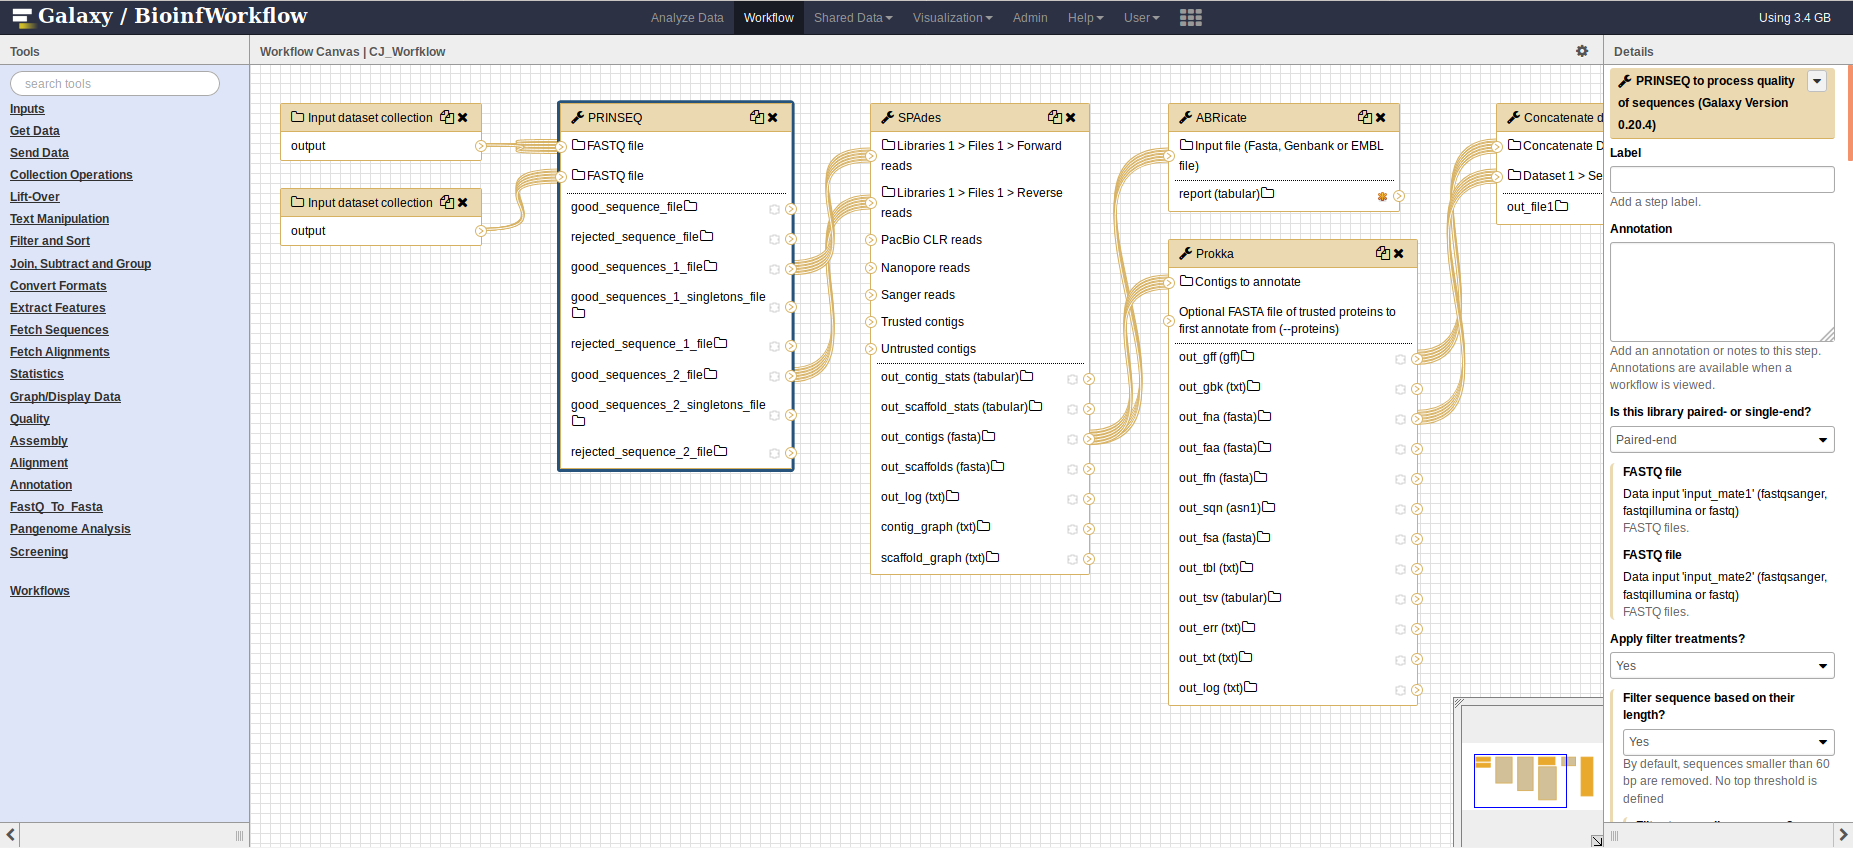
\includegraphics[scale=0.3]{images/InterfazWorkflowEdit.png}
      \caption{Interfaz de edición del workflow}
      \label{fig:WorkflowEdit}
    \end{center}
\end{figure}
Una vez visto el proceso de introducción de datos de entrada, encontramos las herramientas del workflow, cuyo funcionamiento se explica con más profundidad en el \autoref{chap:sistemadesarrollado}: <<Sistema, Diseño y Desarrollo>>. Para modificar los parámetros de cualquiera de las herramientas, podremos seleccionarla y veremos una serie de opciones en la parte derecha de la pantalla, como vemos en la imagen~\ref{fig:WorkflowEdit}. Todos los parámetros modificados ya están guardados en el workflow, pero si se desea cambiar alguno de ellos, se podrá hacer desde esa interfaz. En caso de que se necesite añadir alguna herramienta extra, en el listado de la izquierda se encuentran ordenadas por categorías y con un clic serán añadidas, a falta de enlazar sus ficheros de entrada y de salida con las demás herramientas. Otro aspecto relevante a destacar es que, por defecto, en \textit{Galaxy} los datos se establecen como ocultos a no ser que se marquen con el asterisco que podemos ver a la derecha de los nombres de cada conjunto de datos de salida. Si hacemos clic en ese símbolo, los ficheros ya no aparecerán como ocultos y serán visibles en nuestro historial.

Los historiales son el sistema con el que \textit{Galaxy} ordena los conjuntos de datos del usuario. Desde la página de inicio <<Analyze Data>> podremos consultar el historial activo en este momento  en la parte derecha de la pantalla, pero este no tiene por qué ser el único que existe. Para consultar todos los historiales, desde la propia columna del historial activo, en la parte superior derecha, veremos tres símbolos con las opciones <<Refresh history>>, <<History options>> y <<View all histories>>. Desde esta última accederemos a una nueva pantalla en la que podremos consultar todos los historiales, Es posible que queramos ver conjuntos de datos ocultos de un historial, para ello, podremos activar la opción <<show hidden datasets>> situada debajo del nombre del historial.

Una vez comprendido el funcionamiento del workflow y los historiales, podremos ejecutar el workflow. Para ello, accederemos de nuevo a la pestaña <<Workflow> y desde el desplegable de <<CJ\_Workflow>> seleccionaremos la opción <<run>>. Esto nos situará en una nueva pantalla en la que, de nuevo, podremos modificar todos los parámetros de las herramientas del workflow. Sin embargo, es algo opcional en este momento. El punto principal es la introducción de los datos de entrada, que se seleccionarán desde dos desplegables (uno para cada sentido de las lecturas) en los apartados <<Input dataset collection>>. Si hemos creado las colecciones como se ha explicado previamente, estas aparecerán en el desplegable y solo tendremos que seleccionarlas. El paso siguiente, teniendo en cuenta que no queremos modificar ningún parámetro, será la ejecución del workflow usando el botón <<Run Workflow>> de la parte superior derecha.

A través del uso de los historiales, tendremos la opción de consultar el estado de las ejecuciones de cada una de las tareas del workflow. Teniendo en cuenta los pasos para consultar los historiales explicados anteriormente, podremos ver si una tarea se está ejecutando, en cola, pausada o si ha  causado algún error. Hay que tener en cuenta que es una ejecución computacionalmente muy costosa, por lo que puede llevar varias horas completarla. Por ello, es importante seguir el progreso a través del historial con el objetivo de asegurarnos de que no ha habido ningún error durante el proceso. Cuando todas las tareas se muestren en color verde, el workflow habrá completado su ejecución y podremos descargar los conjuntos de datos resultantes que nos interesen haciendo clic en ellos y seleccionando el icono con la opción <<download>>.

\begin{figure}
    \begin{center}
      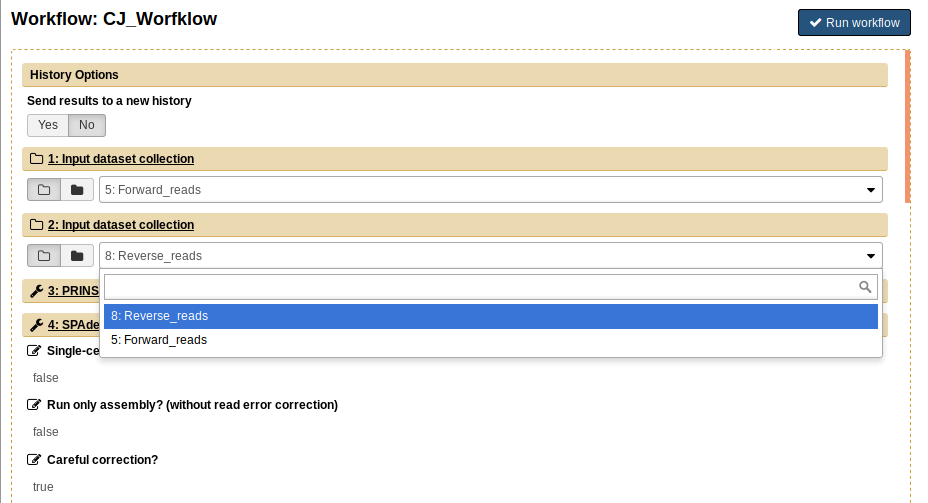
\includegraphics[scale=0.5]{images/RunInputs.png}
      \caption{Selección de las colecciones de entrada del workflow}
      \label{fig:RunInputs}
    \end{center}
\end{figure}

\subsection{Utilidad de ejecución simplificada}
\label{EjecucionSimplificada}
Para facilitar el proceso explicado anteriormente, se ha desarrollado una utilidad que automatiza todos los pasos descritos. En el directorio <<exes>> del proyecto, encontramos un ejecutable llamado <<GalaxyWorkflow>>. Este programa es capaz de cargar los datos de entrada, crear las colecciones, ejecutar el workflow y descargar los resultados en una carpeta local sin necesidad de que el usuario interaccione con \textit{Galaxy}. 

Es necesario conocer algunos comandos para navegar y realizar operaciones básicas con la terminal. En este caso solo veremos los comandos <<ls>>, <<cd>> y <<cp>>, pero es muy recomendable consultar la guía de \textit{Ubuntu} que incluye otros comandos básicos que pueden ser útiles~\footnote{\url{https://help.ubuntu.com/community/UsingTheTerminal}}. Supongamos que nos encontramos en el directorio de nuestro usuario, la ruta por defecto en la que se abrirá nuestro terminal. Si escribimos <<ls>> obtendremos un listado de los directorios y ficheros que nos podemos encontrar~\ref{fig:ls}. Tanto para este comando como para cualquier otro, podremos obtener más información sobre su uso añadiendo <<man>> antes del comando, es decir: <<man ls>>. Si ahora nuestro objetivo es movernos a uno de esos directorios que aparecen en el listado, ejecutaremos <<cd>> y el directorio al que queremos movernos. Por ejemplo, si fuese el escritorio: <<cd Desktop>>. En caso de que necesitemos volver al directorio padre del que nos encontramos ahora mismo usaremos <<cd ..>>.

En principio, se pueden copiar los ficheros directamente utilizando la interfaz gráfica de \textit{Ubuntu} al directorio que deseemos, pero si se quiere usar la terminal, el comando necesario para copiar será <<cp>> y para mover <<mv>>, que funcionan de la misma manera. Un ejemplo para copiar un fichero <<cepa200.fastq>> al escritorio sería
\begin{lstlisting}[language=bash]
    $ cp cepa200.fastq ./Desktop/cepa200.fastq
\end{lstlisting}
y para moverlo 
\begin{lstlisting}[language=bash]
    $ mv cepa200.fastq ./Desktop/.
\end{lstlisting}
Si se quisiese hacer lo mismo para todos los ficheros de determinada extensión, por ejemplo, fastq: 
\begin{lstlisting}[language=bash]
    $ cp *.fastq ./Desktop/
\end{lstlisting}

Por último, veamos como arrancar un ejecutable. Si suponemos que en el escritorio existe un fichero <<run.sh>>, deberemos escribir la ruta hasta ese fichero precedida de un punto. Por ejemplo, si estuviésemos en el directorio comentado anteriormente, ejecutaríamos <<run.sh>> escribiendo
\begin{lstlisting}[language=bash]
    $ ./Desktop/run.sh
\end{lstlisting}
 Si nos encontramos en el mismo directorio que el ejecutable, la ruta hasta ese fichero será simplemente un punto: 
 \begin{lstlisting}[language=bash]
    $ ./run.sh
\end{lstlisting}

\begin{figure}[!h]
    \begin{center}
      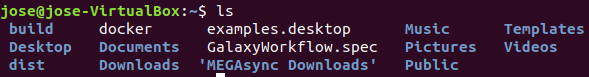
\includegraphics[scale=0.8]{images/ls.png}
      \caption{Ejemplo de un comando ls}
      \label{fig:ls}
    \end{center}
\end{figure}

Pasemos ahora a la utilización del propio workflow. En primer lugar, se requiere que la imagen \textit{Galaxy} esté funcionando y podamos acceder a ella desde el navegador en la dirección <<\url{http://localhost:8080/}>>. Es conveniente realizar esta comprobación antes de ejecutar la aplicación. Si se desea, el usuario puede identificarse como administrador antes de comenzar, para poder consultar lo que está ocurriendo con \textit{Galaxy} mientras la utilidad está funcionando. Es importante dejar claro que interaccionará con dos nuevos historiales, así que para comprobar el funcionamiento, si es que se desea, se deberá hacer desde la vista de todos los historiales.

El proceso para ejecutarlo es muy sencillo, solamente deberemos abrir la terminal de \textit{Ubuntu} y situarnos en el directorio <<exes>> del proyecto. Una vez ahí, veremos que existen dos carpetas <<Forward>> y <<Reverse>>. En ellas deberemos introducir los ficheros \textit{.fastq} de las lecturas que deseamos analizar. Los ficheros de cada sentido de lectura deben dividirse en las dos carpetas. Es necesario que ambas tengan el mismo número de ficheros y muy recomendable que los nombres de los dos sentidos de una lectura comiencen por el mismo identificador único. Por ejemplo, dos nombres de una pareja podrían ser  <<lectura\textbf{1}\_forward>> y <<lectura\textbf{1}\_reverse>>. Cuando contemos con todos los ficheros situados en los directorios correspondientes, escribiremos el siguiente comando.
\begin{lstlisting}[language=bash]
    $ ./GalaxyWorkflow
\end{lstlisting}
Con ello, comenzará la ejecución y cada minuto recibiremos una actualización del estado de las tareas en marcha, pudiendo comprobar si ha habido algún error y ser capaz de detener la ejecución desde \textit{Docker}. Si esto sucediera, la manera más fácil sería detener la imagen \textit{Galaxy} con el comando:
\begin{lstlisting}[language=bash]
    $ ./stop.sh
\end{lstlisting}
O, incluso, resetear la imagen de cero para eliminar todos los ficheros que ya no nos interesan, con la combinación de comandos
\begin{lstlisting}[language=bash]
    $ ./stop.sh
    $ ./remove.sh
    $ ./run.sh
\end{lstlisting}
Normalmente, esto no será necesario y, tras varias horas de ejecución, obtendremos los resultados en un directorio <<ResultsHistory[+timestamp]>> en el que serán ordenados en carpetas dependiendo de la herramienta de la que provengan.

\subsection{Tratamiento de datos obtenidos}
Con la utilidad del apartado anterior, obtenemos un gran número de ficheros independientes. El objetivo de esta herramienta es agrupar los resultados de \textit{ABRicate} y \textit{Roary} en un solo documento \textit{.xls} que podamos abrir como una hoja de cálculo. Para ello, deberemos situarnos de nuevo en el directorio <<exes>>. Nuestros datos de entrada estarán situados en una carpeta con un nombre que comience por <<Results>> y que contenga varias subcarpetas, cada una con el nombre de la herramienta de origen de los ficheros que contiene. Por ejemplo, dos carpetas: <<roary>> y <<abricate>> con los ficheros resultantes de cada una en su interior. Una vez tengamos esta estructura (que por defecto se cumple si se utiliza la herramienta de ejecución automática del workflow) podremos abrir la terminal en el directorio <<exes>> e introducir el comando
\begin{lstlisting}[language=bash]
    $ ./OutputToXls
\end{lstlisting}
Esto generará un fichero con el mismo nombre que la carpeta que hemos indicado anteriormente pero con extensión \textit{.xls} en el que cada hoja del documento corresponderá a una de las herramientas.
\newpage \thispagestyle{empty} % Página vacía 